\documentclass[paper=a4, fontsize=11pt]{scrartcl} % A4 paper and 11pt font size
\usepackage[T1]{fontenc}  % proper encoding for output file
\usepackage[utf8]{inputenc}  % except UTF-8 character in source
\usepackage[english]{babel}  % set document language
\usepackage{amsmath,amsfonts,amsthm}  % math type setting
\usepackage{mhchem}  % chemical expressions
\usepackage{graphicx}  % inclue graphics
\usepackage{url}
\usepackage{caption}
\usepackage{subcaption}
\setlength\parindent{0pt} % Removes all indentation from paragraphs

% Macro to conveniently typeset chemical symbols.
\newcommand{\symb}[1]{$\,\mathrm{#1}$}


% Macro to conveniently typeset chemical symbols.
\newcommand{\symb}[1]{$\,\mathrm{#1}$}

\title{Exercise 2: Vibrational spectra}
\author{Sample Solution}
\date{Effective: 08.11.2018}

%%%%%%%%%%%%%%%%%%%%%%%%%%%%%%%%%%%%%%%%%%%%%%%%%%%%%%%%%%%%%%%%%%%%%%%%%%%%%%%
\begin{document}

\maketitle

1. Find the fundamental band of \symb{CO} and plot its spectrum.
\begin{itemize}
  \item Determine the band center frequency $\tilde{\nu}$ from your plot.
    Figure~\ref{fig:abs_xsec_CO} shows the absorption band of \symb{CO}.
    \begin{itemize}
      \item The center frequency is around
        $\tilde{\nu} = 2143\,\mathrm{cm}^{-1} = 64.2\,\mathrm{GHz}$.
    \end{itemize}

  \item There is some “pollution” in the P-branch that comes from lines
    of \symb{^{13}CO}. Recalculate the spectrum for only the main isotopologue.
    \begin{itemize}
      \item The recalculated spectra for the main isotopologue is shown in
        Figure~\ref{fig:abs_xsec_CO_main}.
    \end{itemize}
\end{itemize}

2. Explore the spectrum of either \symb{H_2O} or \symb{CO_2}. Can you find the
different vibration bands?

Figure~\ref{fig:abs_xsec_overview} shows the absorption bands of both,
\symb{CO_2} and \symb{H_2O}. Those two gases are the main causer of the green
house effect. It shows that both gases are absorbing in different spectral
regions.

The symmetric stretch mode of \symb{CO_2} at 1330\,cm$^{-1}$ is not associated
with a change in the dipole moment, and therefore is not infrared active. The
visible weak bands away from the fundamental frequencies are isotopologue
bands; the isotopologue is no longer symmetric and the fundamental becomes
visible.

\clearpage
\begin{figure}[h!]
  \centering
  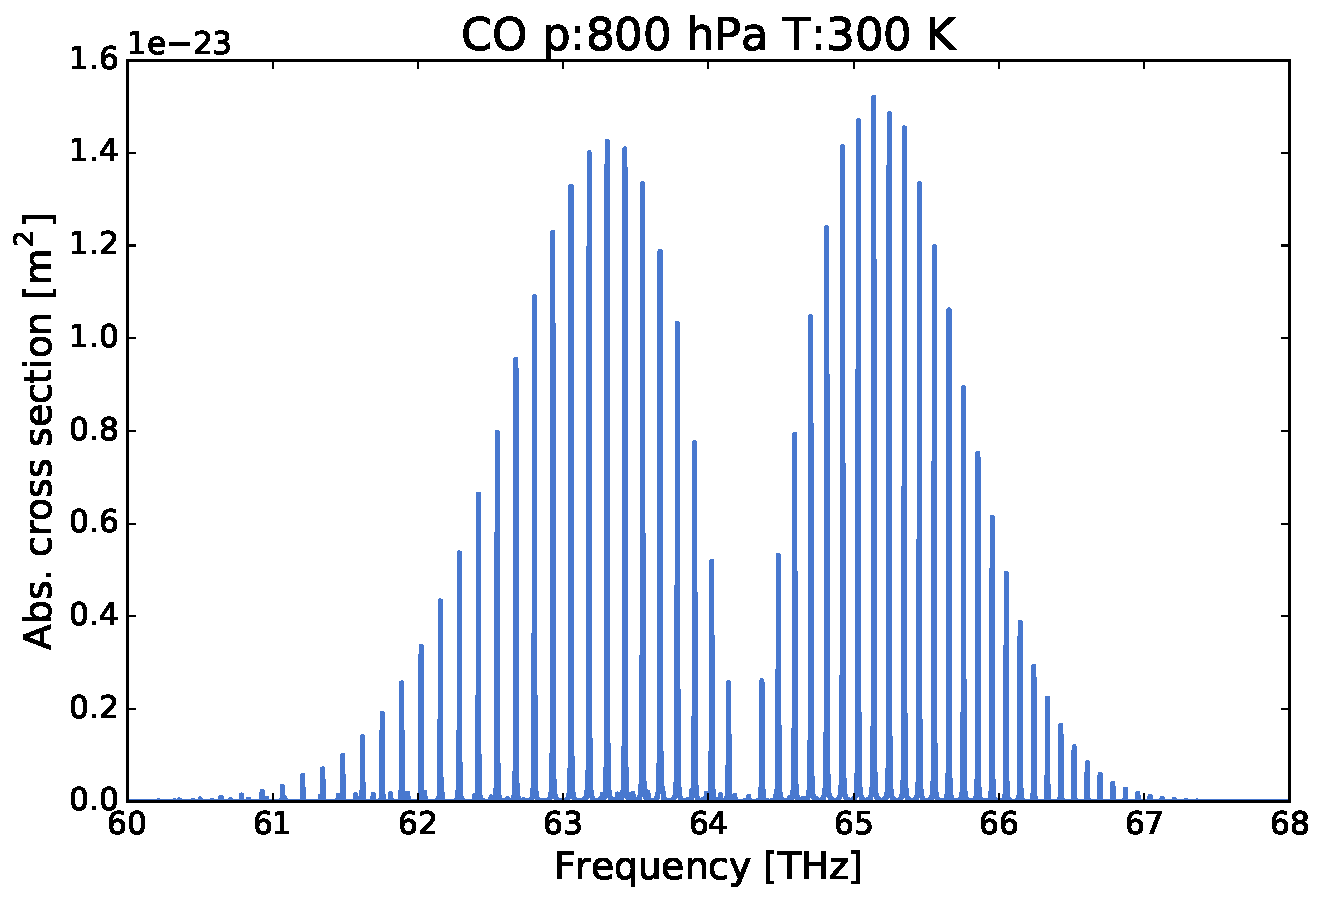
\includegraphics[width=0.8\textwidth]{plots/plot_xsec_CO_800hPa_300K.pdf}
  \caption{Absorption cross section for \symb{CO} (all stable isotopologues).}
  \label{fig:abs_xsec_CO}
\end{figure}
\vfill
\begin{figure}[h!]
  \centering
  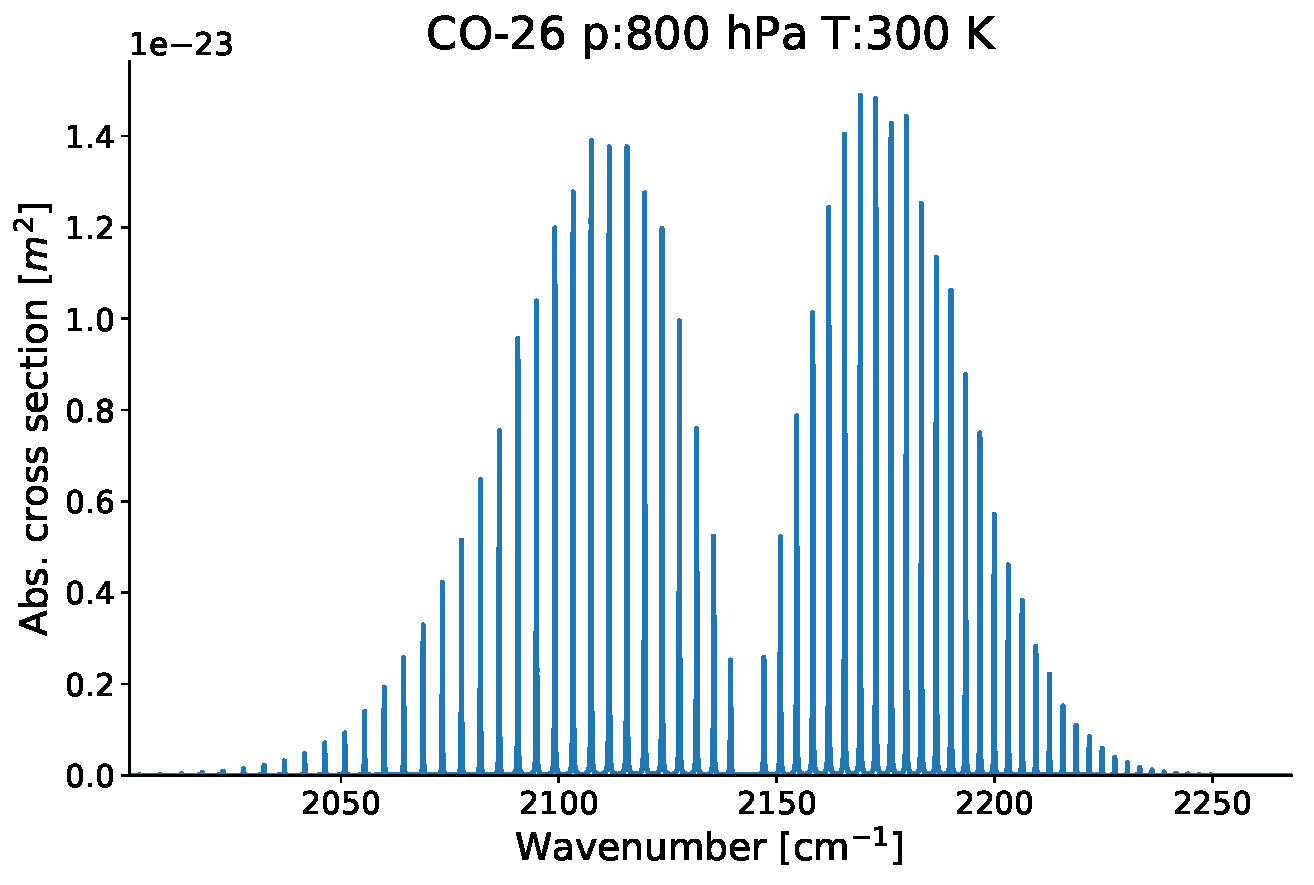
\includegraphics[width=0.8\textwidth]{plots/plot_xsec_CO-26_800hPa_300K.pdf}
  \caption{Absorption cross section for \symb{CO} (main isotopologue).}
  \label{fig:abs_xsec_CO_main}
\end{figure}

\begin{figure}[ht]
  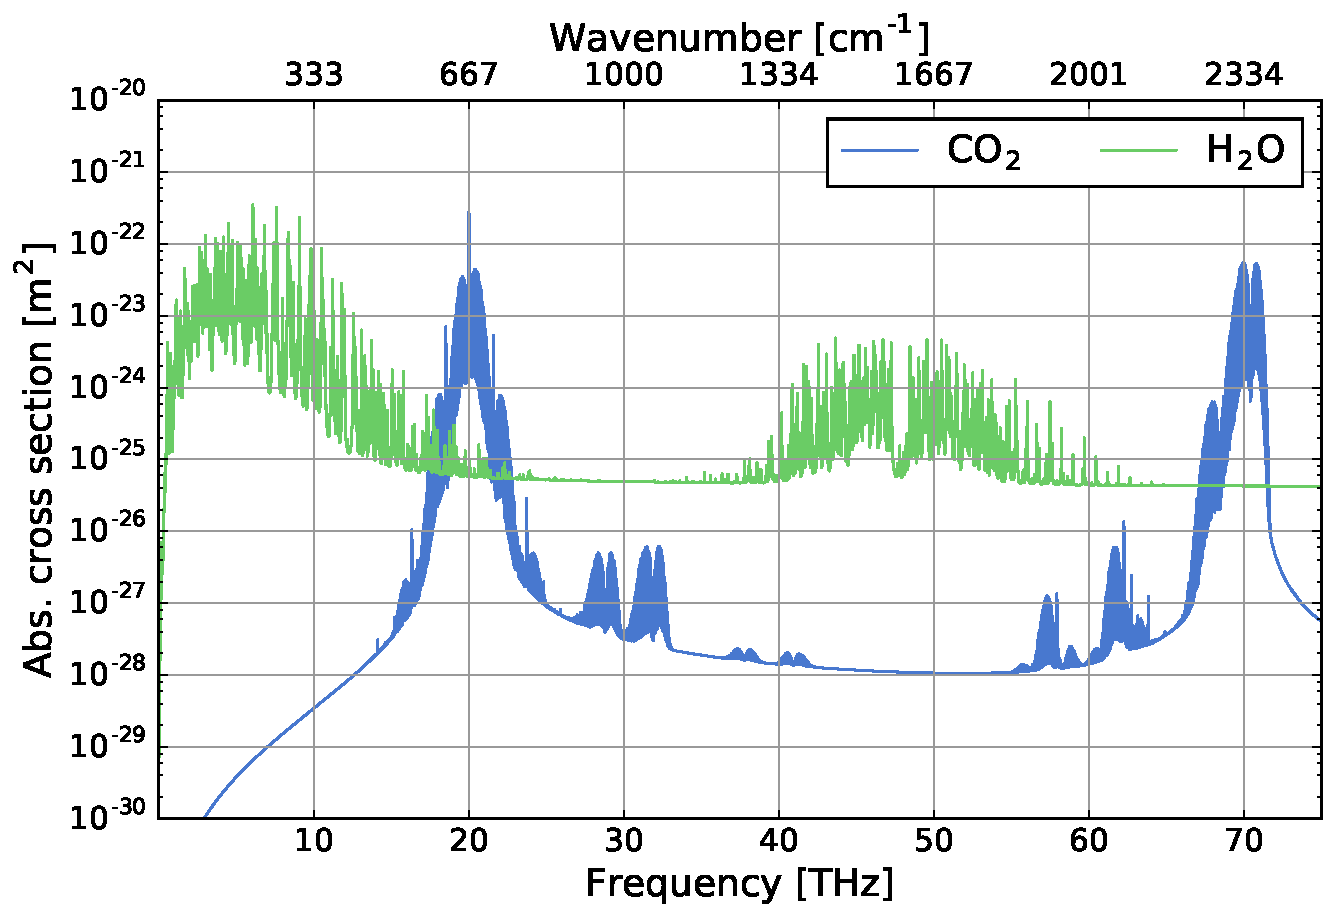
\includegraphics[angle=90, width=0.9\textwidth]{plots/abs_xsec_overview.pdf}
  \caption{Absorption cross sections for \symb{CO_2} and \symb{H_2O}.}
  \label{fig:abs_xsec_overview}
\end{figure}


\end{document}
